\begin{quote}
	\textit{``A vacant-eyed clerk glanced up at me \ldots\ He was wearing a bifocal visor, which gave him a semitransparent view of the OASIS while also allowing him to see his real-world surroundings.''}%~\cite{Cline2012}
\end{quote}
\hfill \textit{Ready Player One, Ernest Cline}
\\
\\
\\

%=========================================================================================================

This chapter discusses the design \& development of a hardware \& software platform which allows its user to observe \& move around their Real World (RW) environment whilst wearing a wide field of view (FOV), stereoscopic 3D, Head Mounted Display (HMD) which allows them to alternatively view an immersive Virtual Reality (VR) environment from the equivalent vantage point. This is achieved by combining a head-tracked HMD, webcams, an indoor positioning system (IPS) \& a 3D game engine, into a mobile PR interface. This project addresses the shortcomings identified in the VTW platform, by using more accurate position tracking, faster \& more responsive orientation tracking \& a more immersive virtual display.

%Previous XR research approached the vacancy problem by integrating sensor/actuator networks into the environments, such that actions in one could manifest in the other, however direct visual engagement with the virtual environment was only possible from static interfaces at pre-determined locations within the real environment~\cite{Lifton2007a, Dublon2011}. The platform discussed in this document addresses this shortcoming by providing a mobile interface for visual engagement with both environments of a XR system, allowing the user to transition between viewing their real environment \& a virtual environment at any time while maintaining the freedom to move around them, multiplexing visual stimuli from their real surroundings \& from a parallel, virtual `mirror world'~\cite{Gelernter1993}.

%=========================================================================================================

%A second example of such a situation is found in the book \textit{Ready Player One}, in a scene in which the protagonist users the equivalent of an Internet cafe to access the \textit{OASIS};

%The OASIS is similar to Snow Crash's Metaverse; a fictional multi-user 3D environment with no enforced likeness to the real world, accessed via \textit{``a visor \& a pair of haptic gloves''}. The bifocal visor allows this character to switch his attention between the virtual environment of the OASIS \& his real surroundings in the Internet cafe.

%=========================================================================================================

\section{Learning from VTW}
The development of the VTW platform as a first foray into applying the concept of PR to the field of virtual heritage was met with concerns, in terms of both quantitative performance \& qualitative experience. Firstly \& most critically, the accuracy of position tracking attainable by using a GPS receiver, even one of higher specification \& real world performance than those commonly found in smartphones, was not sufficient for the envisaged style of interaction. Secondly, the ability of a hand held  display (the tablet) to provide immersive 3D graphics of a complete, atmospheric reconstruction was limited. Moving forward from VTW, a new project was embarked upon to address these concerns with aims to greatly improve the experience of PR in a virtual heritage scenario.

In contrast to VTW, which was intended for outdoor use upon cultural heritage sites where either no remnants or only parts of original structures still stand, the successive platform is intended for use indoors. This not only allows the investigation of the application of PR to cultural heritage to be expanded to indoor scenarios, for sites where more of a historic structure still stands, but also allows for the use of an indoor positioning system, many of which offer substantially more accurate proven real world accuracy than GPS does for outdoor positioning.

Furthermore, in place of a hand held display such as the tablet used by VTW, the successive platform makes use of a head mounted display offering stereoscopic 3D graphics over a wide field of view, that promises much greater immersion, with a head tracking solution that substantially outperforms the orientation tracking employed by VTW both in terms of accuracy \& responsiveness.

%=========================================================================================================

%\subsection{The Mirrorshades Platform}
Figure \ref{systemarchitecture} presents a high level architectural overview of the successive PR platform, dubbed Mirrorshades\footnote{\textbf{Mirrorshades: The Cyberpunk Anthology} (1986) is a defining cyberpunk short story collection, edited by Bruce Sterling. Mirrored sunglasses are a symbol considered synonymous of cyberpunk, a genre whose fiction has frequently involved immersive multi-user virtual environments \& head mounted displays.}. This is a hardware \& software platform which allows its user to observe \& move around their Real World (RW) environment whilst wearing a wide field of view (FOV), stereoscopic 3D, Head Mounted Display (HMD) which allows them to alternatively view an immersive Virtual Reality (VR) environment from the equivalent vantage point. The HMD is imbued with video see-through functionality by the addition of cameras, to allow the user to see their RW environment \& a controller held by the user allows them to trigger their view to switch between RW \& VR.

\begin{figure}[h]
	\begin{center}
		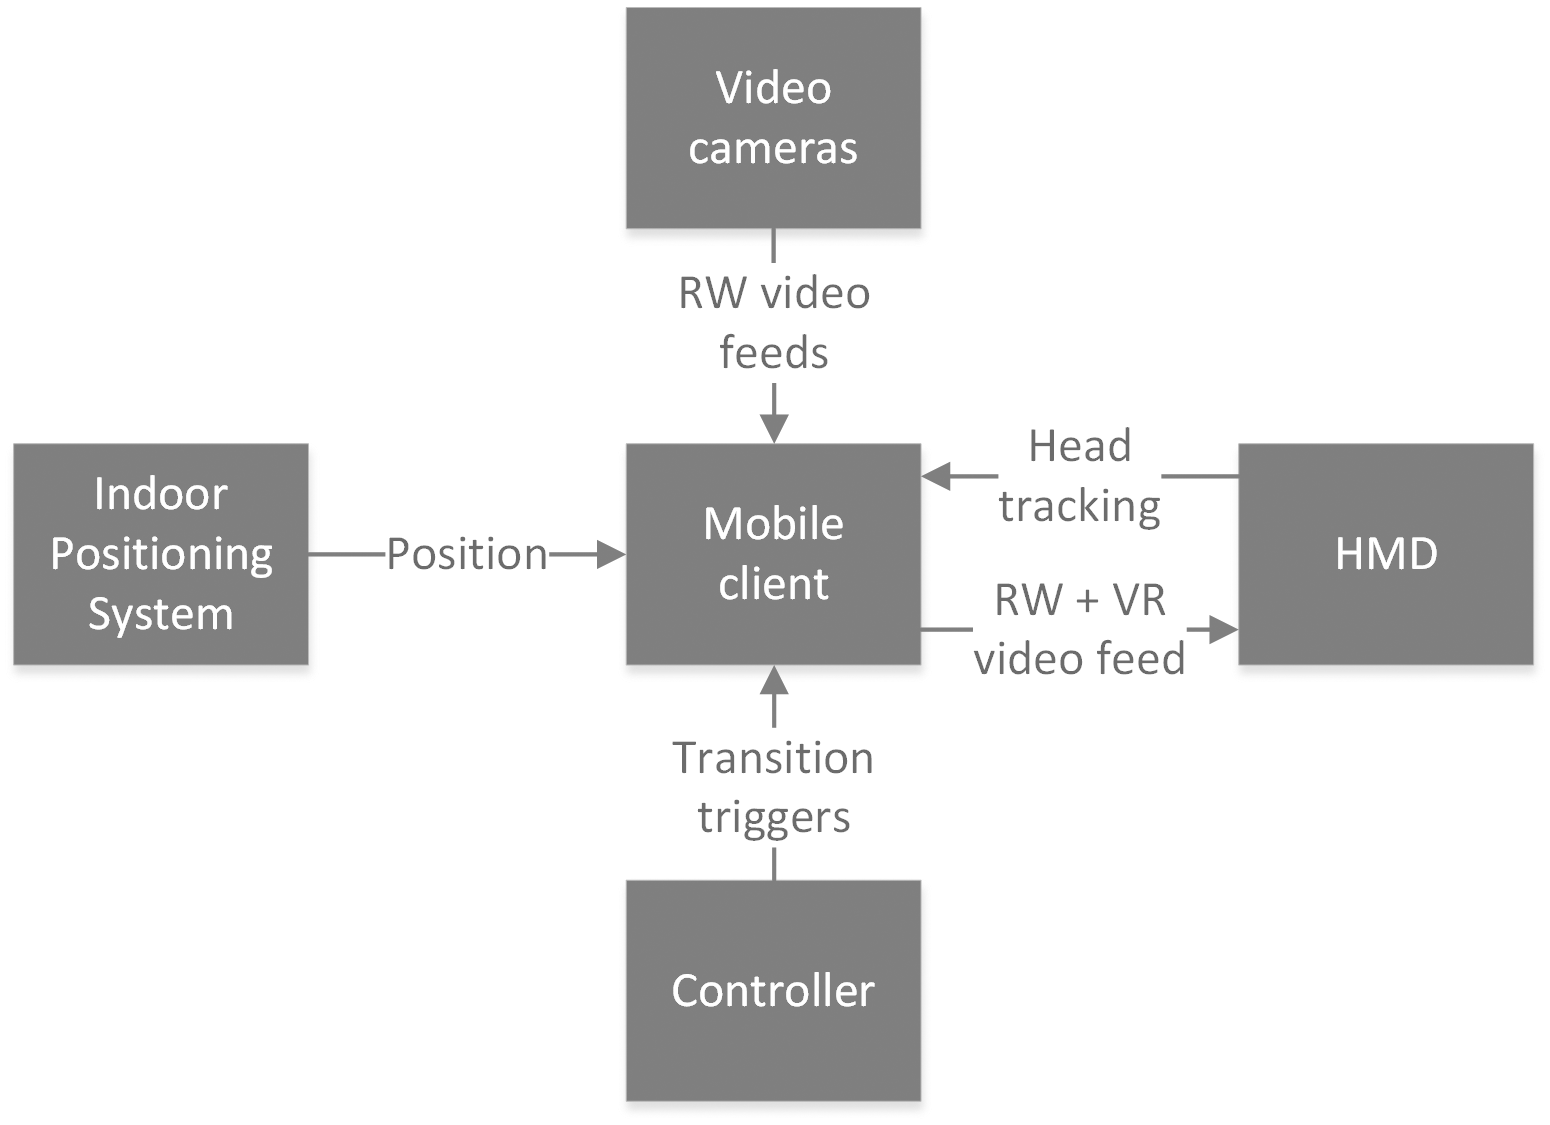
\includegraphics[width=.5\linewidth]{system-architecture.png}
		\caption{Overview of the Mirrorshades platform.}
		\label{systemarchitecture}
	\end{center}
\end{figure}

\textbf{***I think there needs to be some more explanation/diagram/picture of the system here before I start talking about the specifics of the implementation?}

\textbf{***Introduce Sallies as case study/experimental location here?}

%=========================================================================================================

\section{Indoor Positioning Systems}

For outdoor applications, GPS represents a suitable solution for the vast majority of position tracking requirements. Global coverage \& the ability to scale accuracy as required, from many metres with a basic GPS receiver such as those integrated into smartphones, to a few metres with SBAS augmentations \& further to as little as 10cm with the deployment of Differential GPS (DGPS) beacons, has led to GPS occupying the role of the `go to' solution where position tracking is required for an outdoor application. For indoor applications however, there is no single technology or solution that provides similar coverage or suitability as GPS does outside: a large number of different technologies have been employed to produce Indoor Positioning Systems (IPS), which are summarised in figure \ref{mautz-table.png}.

\begin{figure}[h]
	\begin{center}
		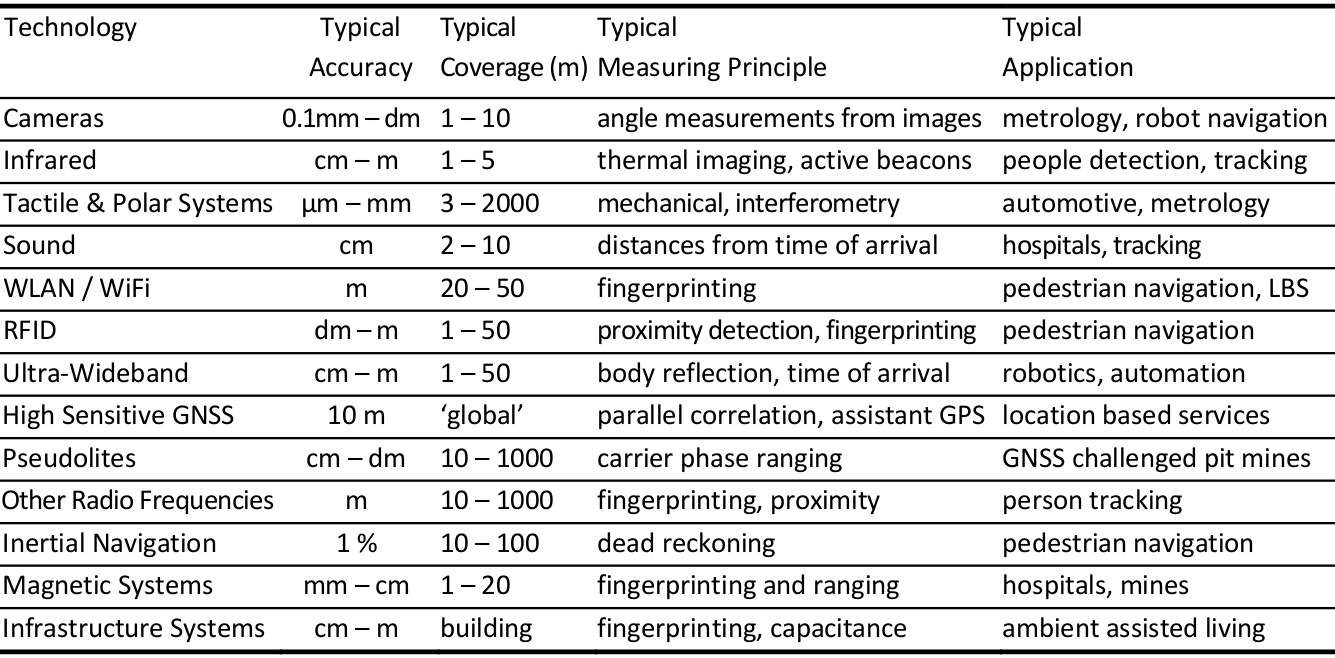
\includegraphics[width=\linewidth]{mautz-table.png}
		\caption{Overview of IPS technologies, from~\cite{Mautz2012}.}
		\label{mautz-table.png}
	\end{center}
\end{figure}

Because of this diversity in technology, with different IPS solutions covering various swathes of the continuums of accuracy \& coverage (see figure \ref{Mautz-000.png}), introducing a host of performance \& suitability considerations, it is necessary to carefully consider the requirements of the application (see figure \ref{Mautz-003.png}) \& then choose the best suited of the many different IPS approaches. Unsurprisingly, selection of a particular IPS usually leads to balancing these requirements in a trade-off, as each of the challenges of indoor positioning effects each technology more or less than others~\cite{Mautz2009}.

\TwoFig{Mautz-000.png}{IPS technologies plotted against their accuracy \& coverage, from~\cite{Mautz2012}.}{Mautz-000.png}
       {Mautz-003.png}{Requirements parameters of IPS, from~\cite{Mautz2012}.}{Mautz-003.png}

%=========================================================================================================

\subsection{IPS Requirements for Mirrorshades}
The positional accuracy of the IPS used for the Mirrorshades platform needs to be substantially higher than that of the GPS solution used for VTW. As a pedestrian application wherein the user walks through doorways (whether real or virtual) \& observes multiple rooms within a building, it is necessary to achieve a level of accuracy that allows, for example, reliably discerning between adjacent rooms, between a doorways \& their surrounding walls \& for approximating position within rooms \& corridors.

Coverage required depends largely upon the size of the cultural heritage site that Mirrorshades is deployed to. However it is prudent to select an IPS that can scale quite arbitrarily from small scenarios (perhaps of a small village church) to substantially larger scenarios (such as a cathedral similar to that at St Andrews), such that the suitability of the platform isn't restricted to sites of particular sizes.

A high update frequency is not especially important to Mirrorshades. The envisaged style of interaction is one wherein users walk relatively slowly through the environments, as they wish to observer \& take in their surroundings. Updates in the range of several hz will be sufficient, especially if users are attending more to their real environment than the equivalent virtual environment when actively moving around (which is to be encouraged, as one cannot walk through a RW obstacle as one can a VR one). Similarly, low latency is not critical. Even if the IPS takes a few seconds to `catch up' with the user, because the user is committed to a deliberate study \& comparison of their real \& virtual surroundings they are not going to be foiled in their task if they find they have to wait momentarily when switching from real to virtual views.

Cost represents a more concrete restriction for Mirrorshades, as the costs of installing \& using different IPS range drastically. For example, an IPS that locates users via propagation modelling/empirical fingerprinting/pathloss of WiFi signals can make use of existing WiFi infrastructure installed in a building \& use nothing more expensive than a smartphone carried by the mobile user. Conversely, using a motion capture suit as an IPS solution will incur substantial costs for each suit, with additional costs for the supporting infrastructure. In a similar vein to the vision of Mirrorshades, an existing project combined the Oculus Rift HMD with an Xsens MVN motion capture suit, allowing participants to walk around a virtual environment of the same layout \& dimensions as their real environment\footnote{\url{https://www.youtube.com/watch?v=LtMfrkRqlRs}}, but without any video see-through of the real environment. The use of a motion capture suit allowed extremely accurate positional tracking, however as a \textit{``complete standard Xsens MVN system is available at around \euro{}50,000''}\footnote{Personal correspondence with Xsens EMEA Entertainment Business Manager.} \& requires a not insubstantial setup phase of the participant donning the suit, it is unsuitable for a virtual heritage scenario where budget is likely to be substantially more limited \&  where visitors are unlikely to be willing to don a complex motion capture suit in order to explore the site. To illustrate a real world comparison of the trade off between costs, accuracy, frequency, etc. of different IPS technologies, considering the departmental building shown by \ref{jack-cole-splodges-black.png}, \textit{``To cover ground floor and have room level accuracy in each room + tracking in the corridors, the cost would be ca. \$25,000''}\footnote{Personal correspondence with Sonitor Technologies Vice President Sales and Business Development EMEA \& APAC.} for a commercial ultrasonic IPS.

Reliance upon deployed infrastructure such as beacons \& markers needs to be avoided for Mirrorshades, as most cultural heritage sites will not allow the installation of any such infrastructure into the site/environment, or may only allow strictly temporary infrastructure to be deployed. Approaches that require extensive infrastructure to be deployed, or for which the deployment \& calibration phase of infrastructure is long \& thus not suitable for temporary deployments, are therefore unusable. Similarly, intrusiveness of the IPS used for Mirrorshades needs to be considered such that the IPS does not drastically affect the user's ability to observe the real \& virtual sites around them.

Robustness of all aspects of a virtual heritage system is critical for enjoyment \& beneficial experience by the user. Visitors to a cultural heritage site, especially if they are only visiting for a short period of time in passing, are not going to be pliant to waiting for a malfunctioning virtual heritage system to right itself. Furthermore, many virtual heritage systems are installed in situations in which the on-site staff do not have the technical knowledge or experience to troubleshoot \& repair them, so these systems must be robust enough to continue successful operation for extended periods of time without intervention by knowledgeable administration.

%http://www.memsic.com/wireless-sensor-networks/MCS-KIT410CA
%8x Crickets
%GBP1850
%email from Willow.co.uk

%=========================================================================================================

\subsection{PlayStation Move}

An initial technology investigated for suitability as an IPS for use with Mirrorshades was PlayStation Move (PSMove), a game controller platform released by Sony for use with their PlayStation 3 console. The platform comprises a hand held controller which contains inertial sensors \& has a plastic sphere on its end that is illuminated from within by a RGB LED. A bundled webcam, the PlayStation Eye (referred to as `PS3 Eye', `PS3Eye' \& `PSEye' among the literature \& community) uses vision tracking to track the controller's position in relation to the camera. Through use of the PSMove API~\cite{Perl2012}, the PSMove platform can be used by a regular computer, by making use of the OpenCV\footnote{\url{http://opencv.org/}} computer vision project.

Whilst the PSMove has been used successfully for pedestrian position tracking in previous projects, included those that used an Oculus Rift HMD\footnote{\url{http://projects.ict.usc.edu/mxr/blog/project-holodeck-wows-in-dublin/}}, it quickly became apparent when auditioning the platform that it only performs reliably when in very dimly lit conditions. Even the relatively dim scene shown by figure \ref{psmove-screenshot.png} (see also ) represented too much ambient light for reliable tracking, so the suitability of the platform for use at a cultural heritage site was removed.

\begin{figure}[h]
	\begin{center}
		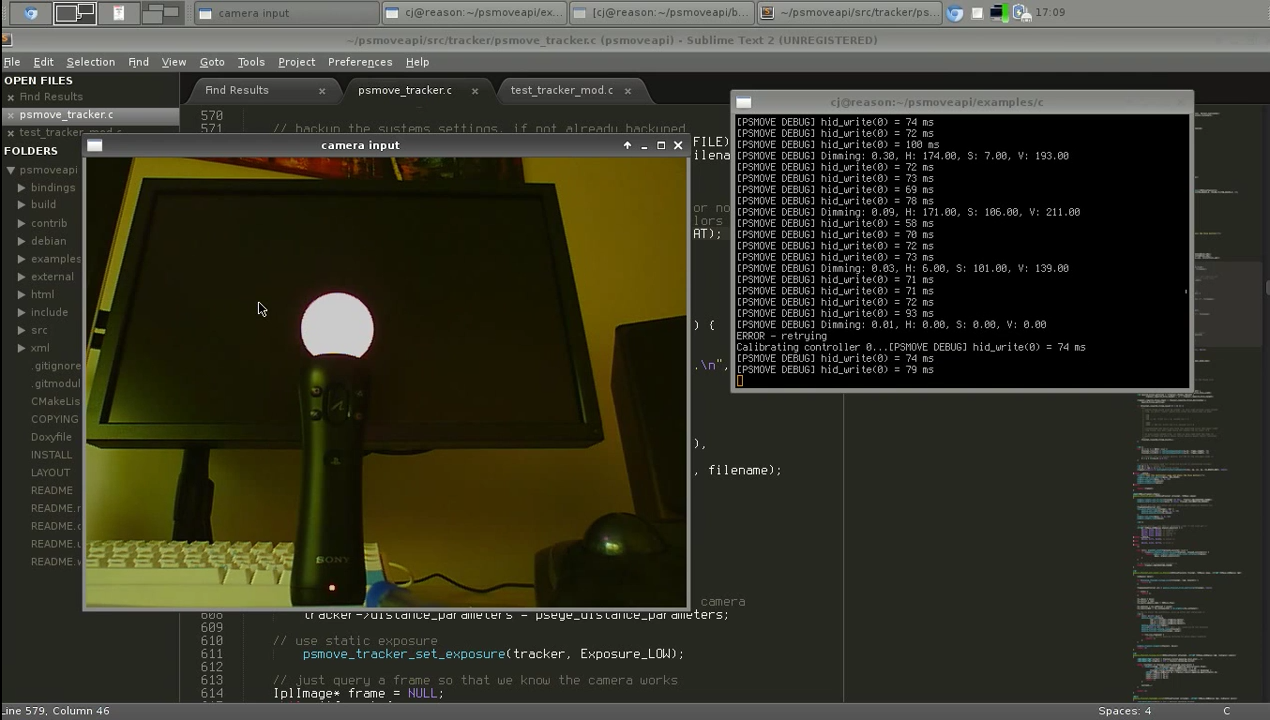
\includegraphics[width=.8\linewidth]{psmove-screenshot.png}
		\caption{PSMove failing to locate even in dim conditions.}
		\label{psmove-screenshot.png}
	\end{center}
\end{figure}

%=========================================================================================================

\subsection{Indoor Atlas}

During the evaluation phase of different IPS \& their suitability to the envisaged Mirrorshades platform, Finnish startup IndoorAtlas\footnote{\url{https://www.indooratlas.com/}} released the first public beta of their indoor positioning technology that uses the magnetometers found in smartphones to locate a user within a magnetic `fingerprint' of a particular building, taking inspiration from animals, such as the spiny lobster, that are able to determine their position as well as their direction from the Earth's magnetic field~\cite{Boles2003}. A spin out from research at the University of Oulu in 2009~\cite{Haverinen2009,Haverinen2009a}, with a similar project undertaken by Media Lab researchers in 2011~\cite{Chung2011}, IndoorAtlas exploits how the Earth's magnetic field is distorted by both natural \& man-made sources. Indoors, these distortions come from building materials, especially in structures employing a framework of metal beams, but also from electrical cabling, HVAC ducting, etc. By recording a map of these distortions in an offline mapping phase, producing a fingerpint of the magnetic field around a building, the location of a user can be deduced by comparing the readings from their smartphone's magnetometer to this fingerprint.

IndoorAtlas promised to be a good match for the IPS requirements of the Mirrorshades platform. In particular, the lack of dependence upon any deployed infrastructure such as ultrasound beacons or visual tracking targets suits the deployment area of Mirrorshades well, as most cultural heritage sites will not be amenable to the deployment of such hardware. Furthermore, the reliance upon only a smartphone held by the user means that coverage is only limited by the area that has prior been mapped in an offline mapping phase, allowing the positioning to scale to arbitrarily large indoor cultural heritage sites. This dependence upon only a smartphone also meets the low cost requirement of the Mirrorshades platform, as mid to high end smartphones with sensitive magnetometers can be purchased for just a few hundred dollars.

The major concern at this point was whether the building materials employed in the construction of cultural heritage sites such as chapels, castles \& cathedrals would create great enough distortions to the Earth's magnetic field for IndoorAtlas to provide its boasted accuracy (which would be sufficient to discern between adjacent rooms, between doorways \& their surrounding walls \& estimate position within rooms \& corridors). These building materials are largely various types of stone, along with wood, a far cry from the metal framework that permeates most modern buildings. Whilst initial tests of the IndoorAtlas beta technology within a departmental building\footnote{\url{https://www.youtube.com/watch?v=l-eIvzpScRs}}\footnote{\url{https://www.youtube.com/watch?v=9hc2zEeQJXQ}} were promising, this was a modern building with a steel beam structure \& an abundance of computing infrastructure \& its associated cabling \& cooling provision. Figure \ref{jack-cole-splodges-black.png} shows the results of one of these tests; the light grey line represents the path walked around the building at a slow walking pace ($<1$ms$^{-1}$, akin to a visitor to a cultural heritage site might walk through it) with each black dot representing a position reported by the IndoorAtlas platform.

It should be noted that the IndoorAtlas technology only reports positions upon routes that have been previously mapped in an offline mapping phase; in figure \ref{jack-cole-splodges-black.png} this offline mapping phase comprised walking the same light grey route several times. In the following test, had the user walked off the light grey route, IndoorAtlas would still have reported the user as being somewhere upon it; it would not attempt to extrapolate their position into unmapped territory. This is presumably because the scale of distortions in the Earth's magnetic field is quite fine grained, supported by the fact that many of the black dots are less than a meter apart, thus extrapolation would not fair well. This is an important aspect to take into account when performing the offline mapping phase, as one must map sufficient paths to cover all possible places \& routes that a user may walk. For locations comprised mainly of corridors \& small rooms, this is not an issue, however for a location that contains a large open space in which the user is free to meander, a more involved mapping process in which the entire space is systematically covered by back \& forth routes that progress across the space is required.

\begin{figure}[h]
	\begin{center}
		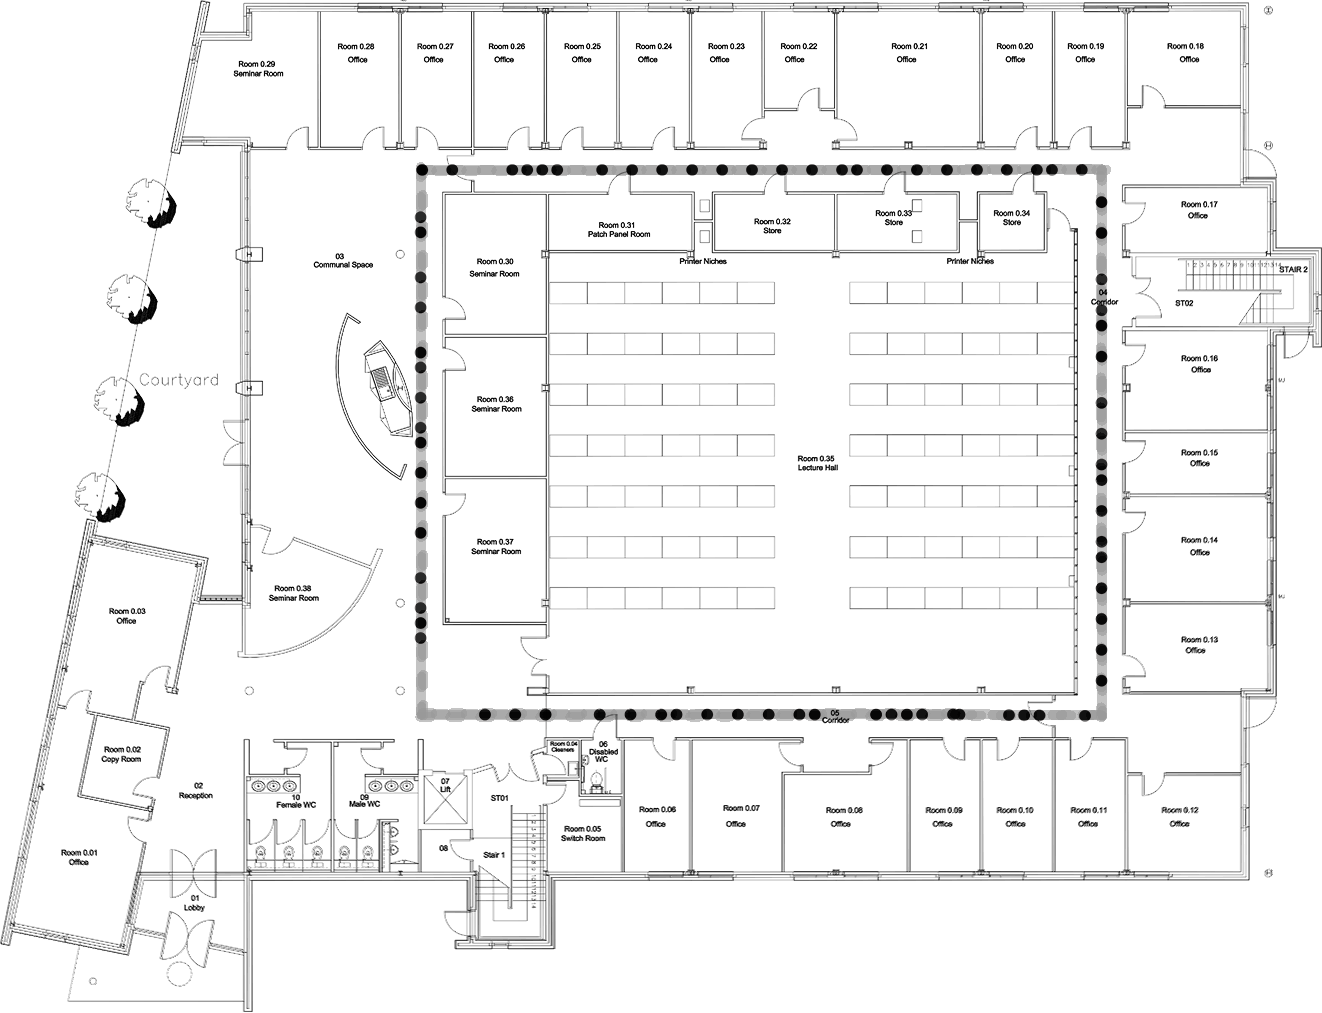
\includegraphics[width=0.7\textwidth]{jack-cole-splodges-black.png}
		\caption{Testing of IndoorAtlas in a department building, approximately 40m wide by 30m tall.}
		\label{jack-cole-splodges-black.png}
	\end{center}
\end{figure}

Initial testing of IndoorAtlas at a 15th century chapel proved surprisingly successful, with the platform able to track the smartphone accurately throughout the building even without any obvious overbearing metal content in the structure or furnishing. Figure \ref{sallies.png} shows the set of positions reported by the IndoorAtlas platform whilst walking throughout the chapel, which is roughly 30m across. Upon closer inspection of the building, metal grating that runs along the ground along the central nave (representing much of the horizontal movement in figure \ref{sallies.png}) might help to explain this unexpected performance, however in other areas such as when walking to either side of the altar there were no obvious sources of magnetic interference to account for the maintained accuracy. Possible hidden explanations could be the ferromagnetic properties of certain types of stone \& the electrical lighting \& audio systems installed into the chapel, which make use of electrical cables routed throughout the building.

\begin{figure}[h]
	\begin{center}
		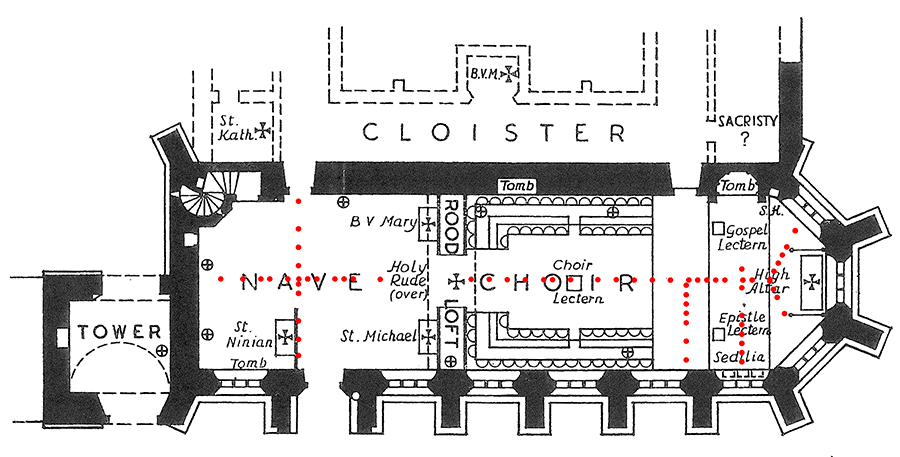
\includegraphics[width=0.7\textwidth]{sallies.png}
		\caption{Testing of IndoorAtlas in a 15th century chapel.}
		\label{sallies.png}
	\end{center}
\end{figure}

\textbf{***Photos of metal grate along nave \& of altar showing not much obvious metal.}

%=========================================================================================================

\section{HMD with See-Through Video}
The concept of virtual reality \& the associated head mounted displays that provide stereoscopic 3D graphics coupled with head tracking are currently experiencing a resurgence of interest \& investment, thanks largely to the advent of Oculus \& their Rift platform.

%1965 The Ultimate Display
%1968 demonstrated the Sword of Damocles

%Virtual Reality - Rheingold, 1992 - 'revolutionary technology...how it promises to transform society'
%\cite{Rheingold1992}


Whilst the first head mounted computer display was created back in the 1960s by Ivan Sutherland, it was not until the late 1980s \& early 1990s that VR began to be pushed to the consumer. Unfortunately, both the hardware \& software was not ready for consumer release \& the systems failed to live up to the substantial hype, resulting in the VR bubble bursting in the 1990s.

After this disappointment, Oculus now looks set to finally begin realising a successful consumer VR platform, thanks largely to substantial advances in display technologies during the past decade, driven largely by the explosive popularity of smartphones \& tablets. Pre-Oculus HMDs largely made use of two separate microdisplays, one for each eye. Sutherland's original Sword of Damocles made use of two micro CRT screens, whilst later HMDs made use of OLED displays. As the number of market applications for microdisplay technology was (\& continues to be) relatively small, this meant that these headsets had a limited number of displays to choose from \& that they were relatively expensive.




late 1980s \& early 1990s that the appeal of VR began to enter the mainstream



The Oculus Rift takes a different approach. Instead of using two small displays, one for each eye, it uses a single larger display upon which two separate images are rendered, side-by-side. This approach has two distinct advantages compared to prior dual display techniques. Firstly, the complexity of the device is reduced. Secondly, the cost of a single display in the 5"-7" size is drastically lower than the cost of a pair of OLED microdisplays, largely thanks to the surging popularity of smartphones \& tablet computers.

The larger size of the display adopted by the Oculus approach also allows for a far greater field of view (FOV) than the microdisplay approach.

Examples of consumer-grade commercial HMDs that use the twin OLED microdisplay approach, the Sony HMZ-T1, which launched with a price of \textyen60,000 (\$800 at exchange rates of the time) \& its successor the HMZ-T2 which launched with a price of \textyen70,000 (\$900 at exchange rates of the time), provided $45\textdegree$ horizontal FOV/$51.6\textdegree$ diagonal \& no head tracking, intended primarily as a personal 3D cinema experience.



In comparison, the first Oculus Rift development kit (DK1) launched at a price of \$300, providing over $90\textdegree$ horizontal FOV/$110\textdegree$ diagonal



Talk about the resurgence of VR thanks to the Oculus Rift \& how it has brought a cheap, wide FoV, fast head tracked, HMD to market for researchers \& enthusiasts.

Brief history of VR headsets, maybe take bits from that youtube video from Samsung developers?

%=========================================================================================================

\subsection{Modifying the Oculus Rift for Stereoscopic See Through Video}

\textbf{***Mention first Mirrorshades test with single webcam providing small floating window in corner of virtual view (video is on youtube/Mirrorshades repo).}

\newcommand{\floatingwebcamFootnote}{\footnote{\url{https://www.youtube.com/watch?v=tS0FGZxQzCU}}}

\begin{figure}[h]
	\begin{center}
		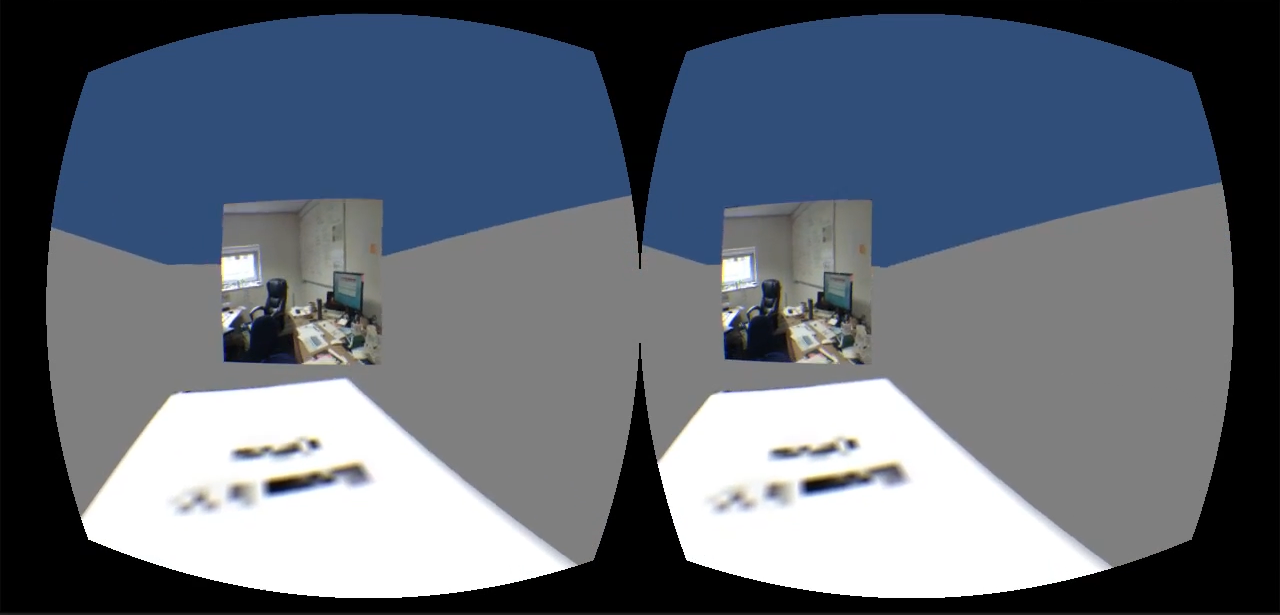
\includegraphics[width=0.7\textwidth]{floating-webcam-window.png}
		\caption{Early floating window Rift/webcam prototype.}
		\label{floating-webcam-window.png}
	\end{center}
\end{figure}

\textbf{**Show lens comparison picture from blog \& a (new?) screenshot showing FoV of the camera feeds compared to that of Rift \& explain why the discrepancy doesn't matter, especially when the Rift is fully extended.}

\begin{figure}[!htb]
    \centering
    \begin{minipage}{.32\textwidth}
        \centering
        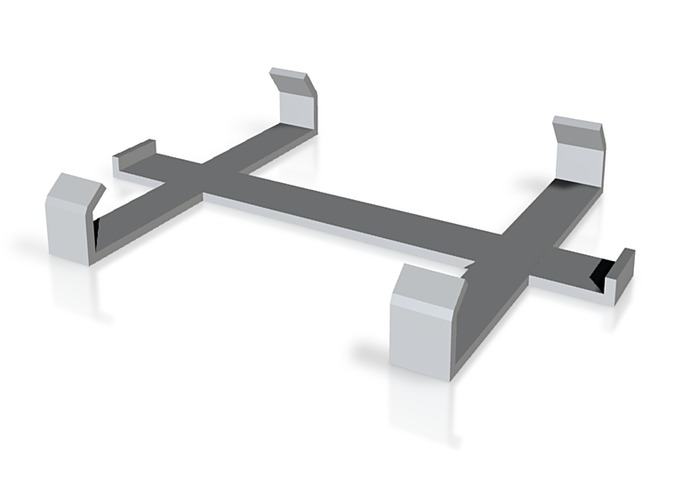
\includegraphics[width=\textwidth]{rift-clips-cameras/clips.jpg}
        \caption{bar}
        \label{bar}
    \end{minipage}%
    \hspace{.01\textwidth}
    \begin{minipage}{0.32\textwidth}
        \centering
        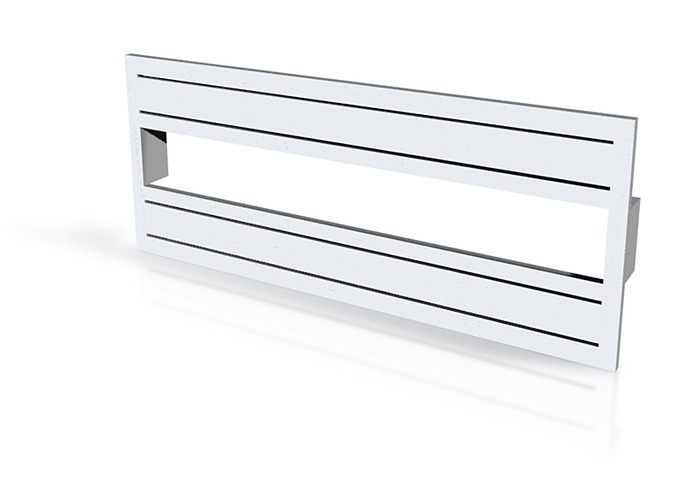
\includegraphics[width=\textwidth]{rift-clips-cameras/clips-hori-plate.jpg}
        \caption{foo}
        \label{foo}
    \end{minipage}%
    \hspace{.01\textwidth}
    \begin{minipage}{0.32\textwidth}
        \centering
        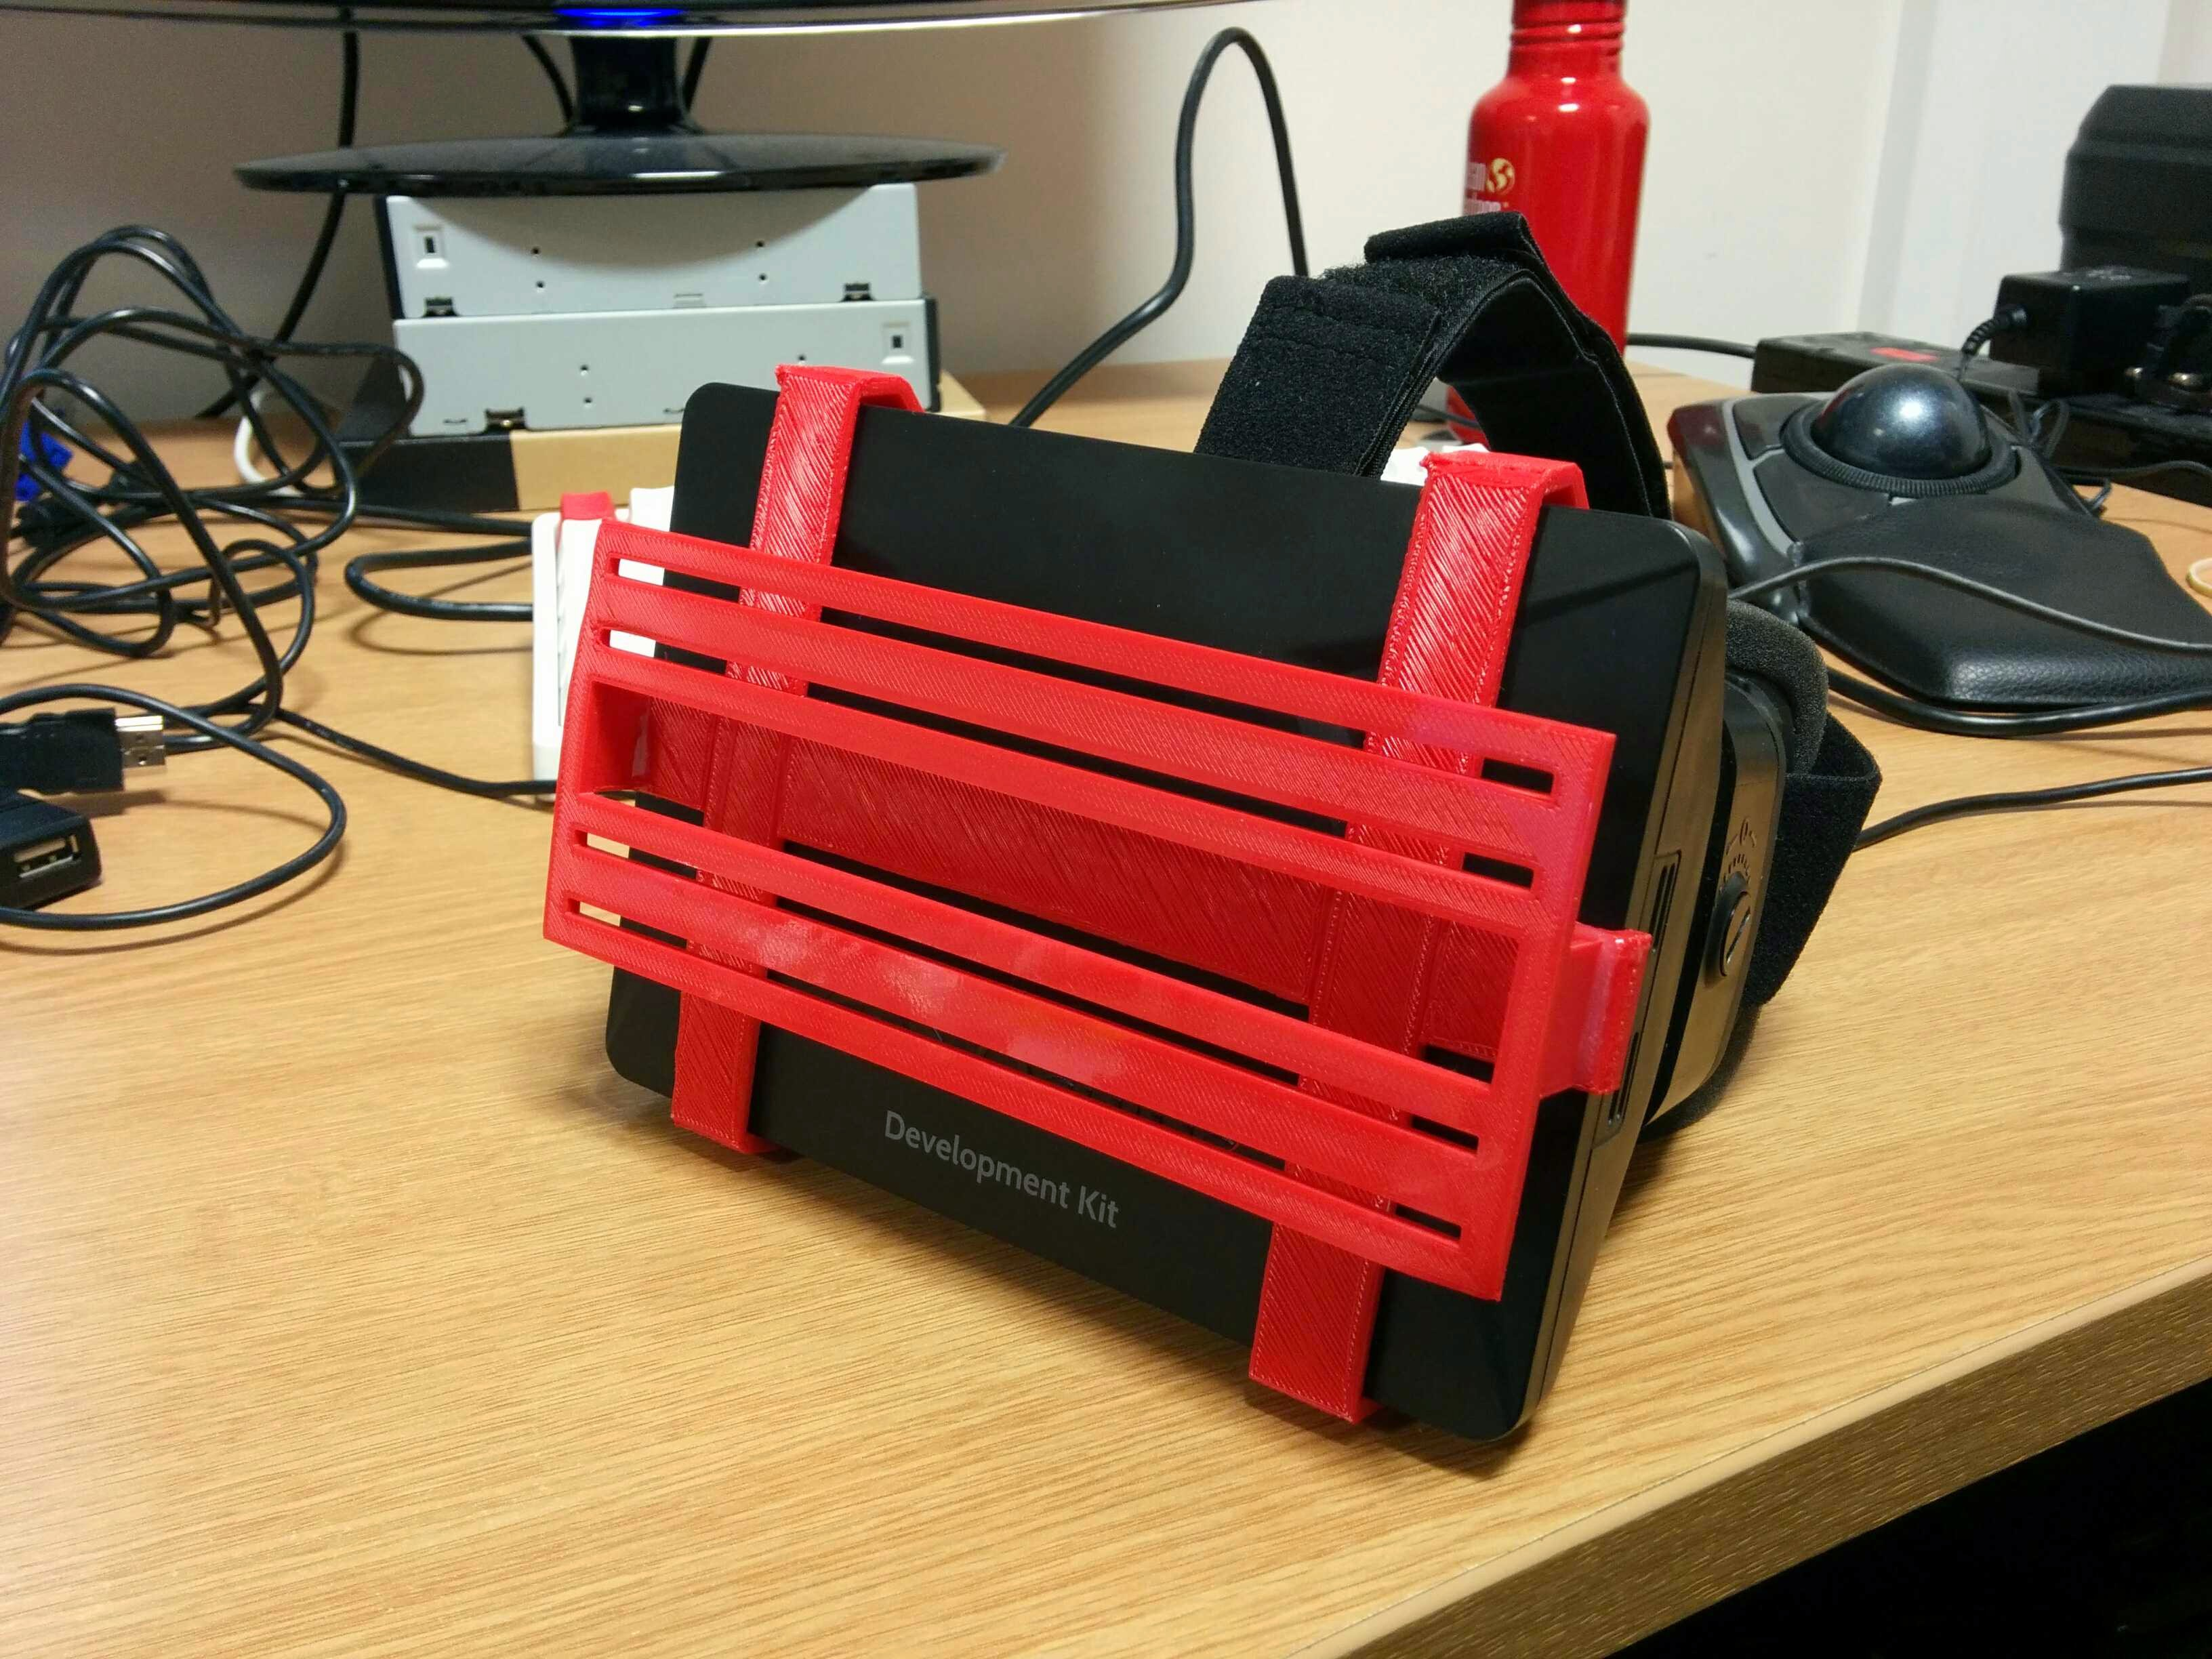
\includegraphics[width=\textwidth]{rift-clips-cameras/hori-1.jpg}
        \caption{baz}
        \label{baz}
    \end{minipage}
\end{figure}

\TwoFig{rift-clips-cameras/hori-2.jpg}{hori-2.jpg}{hori-2.jpg}
       {rift-clips-cameras/hori-3.jpg}{hori-3.jpg}{hori-3.jpg}

\TwoFig{rift-clips-cameras/lens-comparison-on-ps3eye-pcb.jpg}{lens-comparison-on-ps3eye-pcb.jpg}{lens-comparison-on-ps3eye-pcb.jpg}
       {rift-clips-cameras/lens-comparison.jpg}{lens-comparison.jpg}{lens-comparison.jpg}

\TwoFig{rift-clips-cameras/clips-vert.jpg}{clips-vert.jpg}{clips-vert.jpg}
       {rift-clips-cameras/vert-6.jpg}{vert-6.jpg}{vert-6.jpg}

\TwoFig{rift-clips-cameras/vert-1.jpg}{vert-1.jpg}{vert-1.jpg}
       {rift-clips-cameras/vert-4.jpg}{vert-4.jpg}{vert-4.jpg}

\TwoFig{rift-clips-cameras/thermoplastic.jpg}{thermoplastic.jpg}{thermoplastic.jpg}
       {rift-clips-cameras/vert-7.jpg}{vert-7.jpg}{vert-7.jpg}

\TwoFig{rift-clips-cameras/middle.jpg}{middle.jpg}{middle.jpg}
       {rift-clips-cameras/right.jpg}{right.jpg}{right.jpg}

\TwoFig{latency/vid1.jpg}{vid1.jpg}{vid1.jpg}
       {latency/vid2.jpg}{vid2.jpg}{vid2.jpg}

\TwoFig{latency/vid3.jpg}{vid3.jpg}{vid3.jpg}
       {latency/vid4.jpg}{vid4.jpg}{vid4.jpg}

\begin{figure}[h]
    \begin{center}
    \begin{minipage}{.32\textwidth}
        \begin{center}
        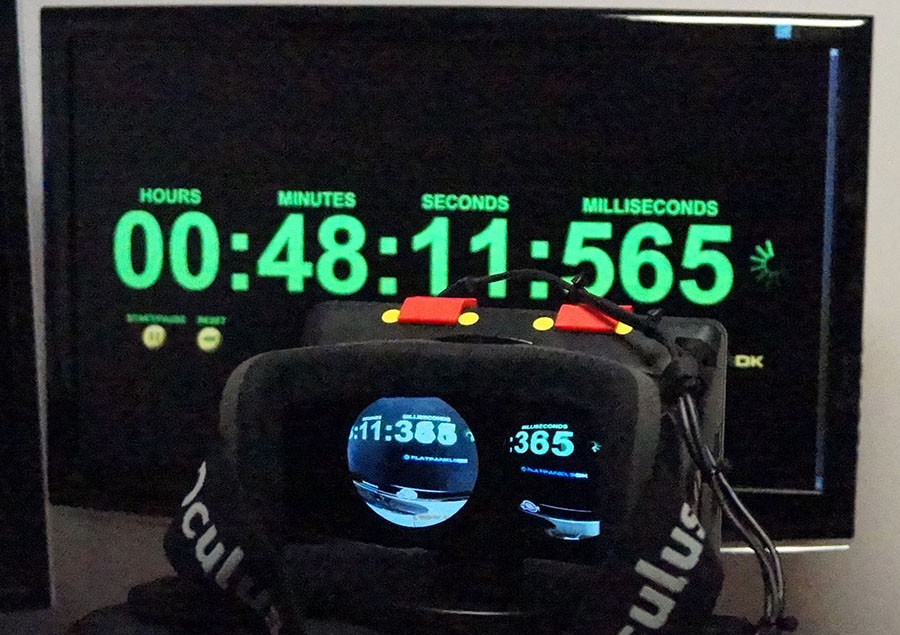
\includegraphics[width=\textwidth]{latency/still1.jpg}
        \caption{still1.jpg}
        \label{still1.jpg}
        \end{center}
    \end{minipage}%
    \hspace{.01\textwidth}
    \begin{minipage}{.32\textwidth}
		\begin{center}
        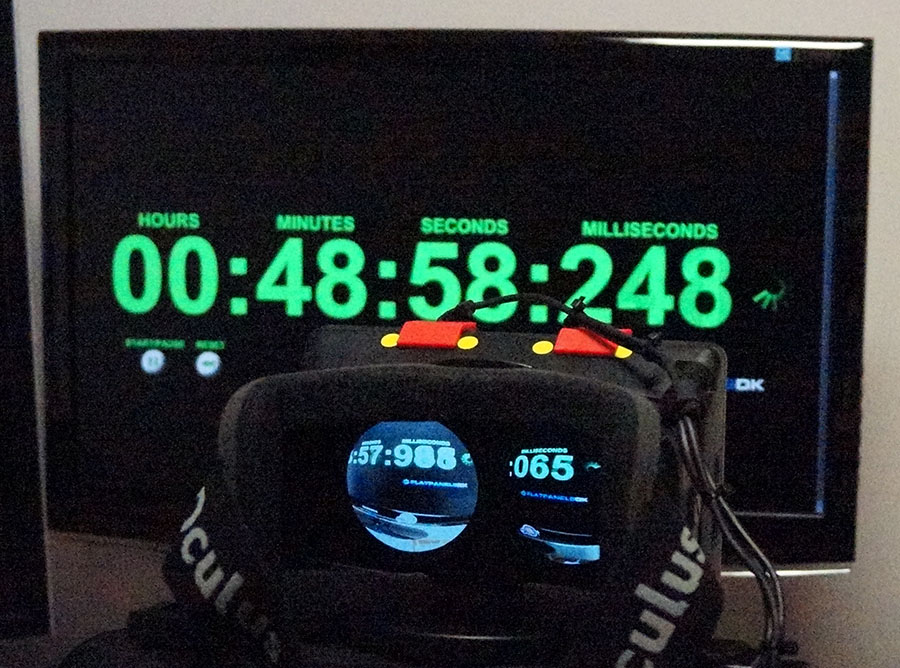
\includegraphics[width=\textwidth]{latency/still2.jpg}
        \caption{still2.jpg}
        \label{still2.jpg}
        \end{center}
    \end{minipage}%
    \hspace{.01\textwidth}
    \begin{minipage}{.32\textwidth}
        \begin{center}
        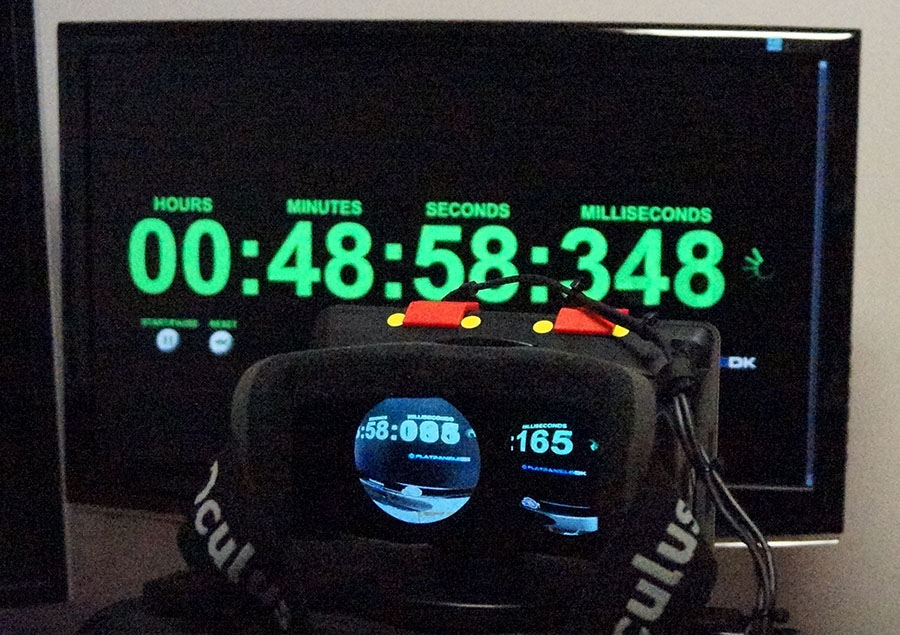
\includegraphics[width=\textwidth]{latency/still3.jpg}
        \caption{still3.jpg}
        \label{still3.jpg}
        \end{center}
    \end{minipage}
    \end{center}
\end{figure}

%=========================================================================================================

\section{Mobile Client}

Talk about trying Oculus on Android (ODROID) \& how now Samsung Gear VR would be ideal, but yolo laptop in a bag. Photo of ODROID/screencap of (\& link to) video showing Rift working (at least tracking) with ODROID?

Talk about ease of Unity integration with Oculus at the time (UE4 wasn't really on the scene?).

%=========================================================================================================

\subsection{Implementation}
Figure \ref{experimentalimplementation} presents an overview of the implementation of the Mirrorshades platform design for use in the chapel investigations.

\begin{figure}[h]
	\thispagestyle{empty}
	\begin{center}
		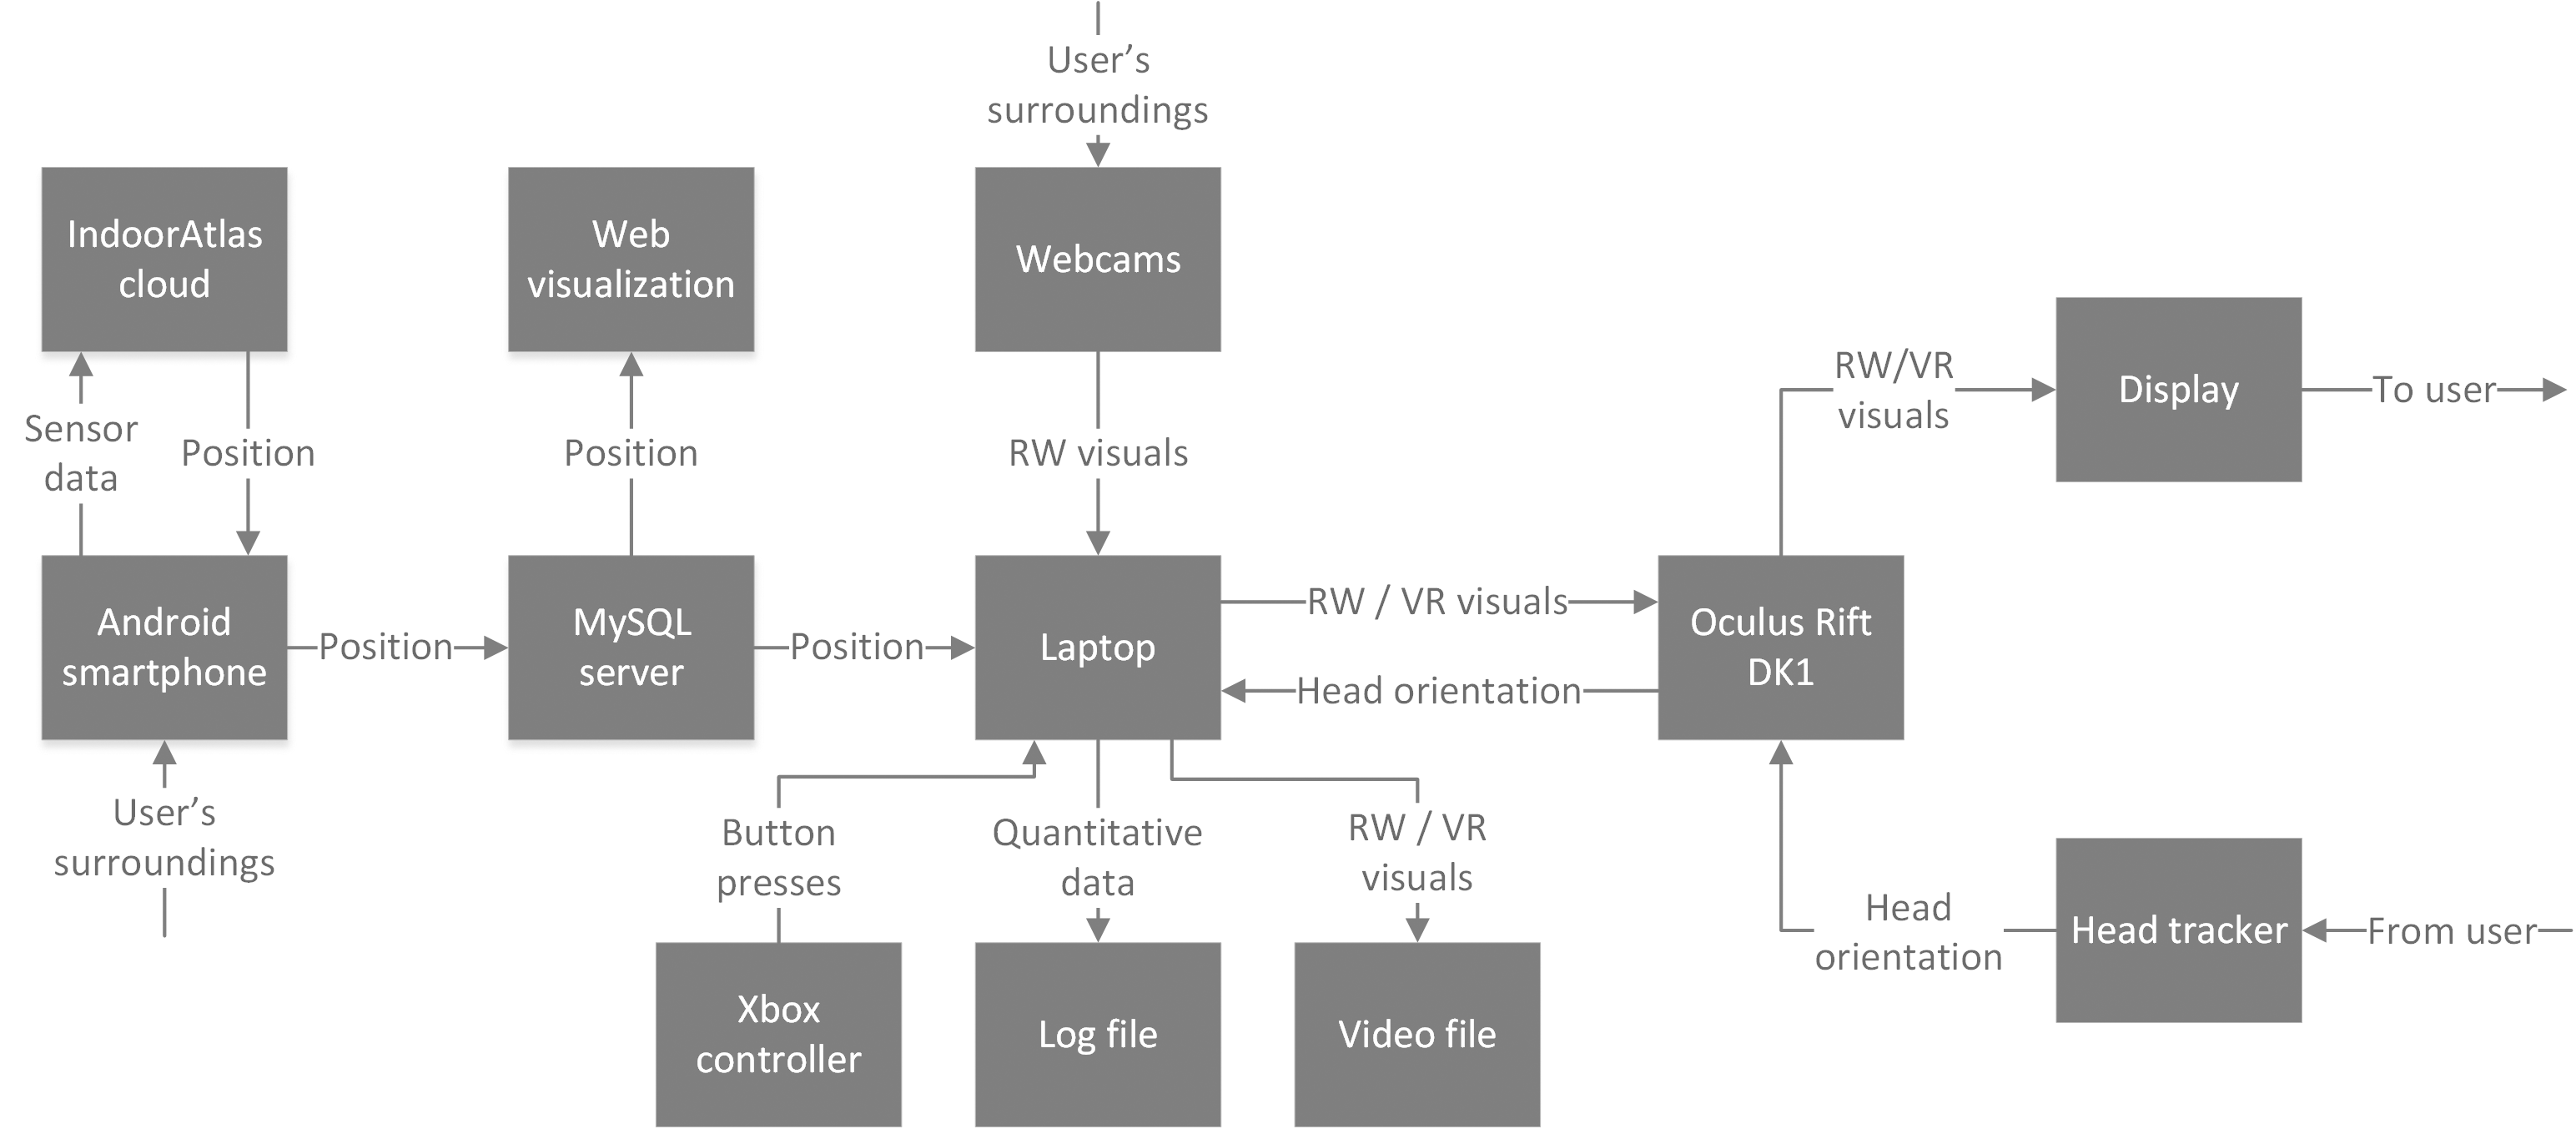
\includegraphics[width=.925\linewidth]{experimental-implementation.png}
		\caption{Implementation of Mirrorshades platform.}
		\label{experimentalimplementation}
	\end{center}
\end{figure}

%=========================================================================================================

\subsection{Hardware Components}
The hardware of the implementation comprises;

\begin{itemize}
	\item an Oculus Rift DK1 HMD, including a 9-axis (3dof rotational) head tracker sampling at 1000Hz \& mounted with a stereo camera solution comprising 2x Logitech C310 webcams modified with M12 lens mounts \& 2.1mm lenses to provide approximately 87 degrees horizontal FOV of the RW environment (see figure \ref{rift});
	\item a USB battery pack, to power the HMD;
	\item a small laptop computer, with an Intel i7-3632QM processor, Nvidia GT 650M graphics card \& 16GiB system memory;
	\item an Android smartphone, running Android 4.4.4;
	\item an Xbox 360 wireless controller, with USB receiver.
\end{itemize}

%\begin{figure}[h]
%	\begin{center}
%		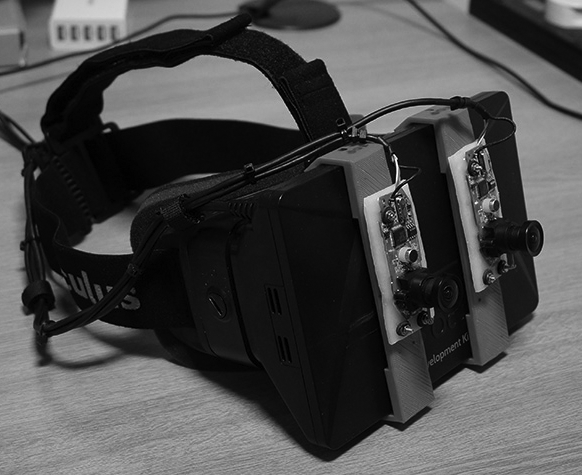
\includegraphics[width=0.6\textwidth]{rift.png}
%		\caption{HMD with stereo camera solution.}
%		\label{rift}
%	\end{center}
%\end{figure}

%=========================================================================================================

\subsection{Software Components}
The software of the implementation comprises;

\begin{itemize}
	\item an Android application that runs on the smartphone, determines the location of the phone within the building that it is in using the IndoorAtlas IPS~\cite{IndoorAtlasLtd.2012} (figure \ref{sallies_layout} shows the paths within the chapel upon which the IPS has been configured) \& submits these location data via PHP to a database server;
	\item a MySQL database server that stores location data for the phone \& allows these data to be accessed both by the Unity application running upon the laptop \& by a web visualisation;
	\item a Unity application that runs on the laptop.
\end{itemize}

%=========================================================================================================

\subsection{Integration of Components}
The Unity application hosts the VR representation of the chapel \& takes in feeds from both webcams, the HMD head tracker \& the Xbox controller. It also polls the database server for the most recent position data. All of these inputs are combined together to form the visual output for the HMD to display to the user.

As the user moves their head, the visuals that are presented to them upon the HMD's display change accordingly; the RW visuals change due to the webcams being physically fixed to the HMD \& the VR visuals change due to data from the head tracker being used to change the orientation of the in game `cameras' accordingly.

As the user changes their position by walking, the visuals that are presented to them upon the HMD's display also change accordingly; again the RW visuals change due to the webcams' position upon the HMD whilst the VR visuals change due to the user's position, as reported by the smartphone \& the IndoorAtlas solution, being used to move the position of the in game cameras to the equivalent position within the VR representation.

As the user presses buttons or pulls triggers upon the Xbox controller, the visuals that are presented to them upon the HMD's display transition between RW \& VR in different styles depending upon which button/trigger was activated.

%=========================================================================================================

\subsection{Transition Methods}
Attending to visual stimuli from the RW environment via the webcams is required for the user to safely move around. Delay in the IPS reporting their position \& inaccuracies in these position data (see figure \ref{jack-cole-splodges} for a set of example position data) mean that moving around while attending only to visual stimuli from the VR environment would not be safe for the user, even with unchanging RW obstacles with perfectly accurate representations in the VR environment. Furthermore it is actually likely that RW obstacles will not have equivalent VR representations, such as in a scenario where XR is used to compare \& contrast changes to a building's interior over extended periods of time (such as with the chapel investigations).

Thus the HMD displays the feeds from the webcams as default \& the user must trigger transitions to view the VR environment by pressing a button or pulling a trigger on the controller. Releasing the button/trigger causes the webcam feeds to be displayed again.

%=========================================================================================================

\subsubsection{Hard switch}
\label{sub-hardswitch}
The user presses \& holds the \texttt{[A]} button on the controller to switch the visual stimuli displayed by the HMD from RW to VR. When the \texttt{[A]} button is released, the visual stimuli displayed by the HMD switch back from VR to RW. This is a `hard' or `immediate' switch with no fading or transition effect. Figure \ref{scenario1} illustrates this scenario.

\begin{figure}[h]
	\begin{center}
		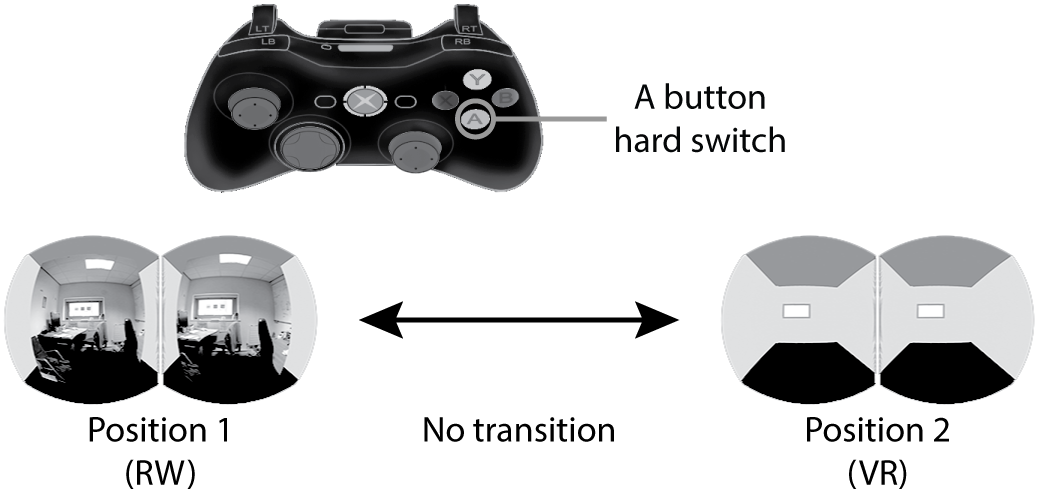
\includegraphics[width=0.7\textwidth]{switching-hard-with-controller.png}
		\caption{Hard switch.}
		\label{scenario1}
	\end{center}
\end{figure}

%=========================================================================================================

\subsubsection{Switch with linear interpolation}
The user presses \& holds the \texttt{[B]} button on the controller to switch the visual stimuli displayed by the HMD from RW to VR. When the \texttt{[B]} button is released, the visual stimuli displayed by the HMD switch back from VR to RW. This switch fades between RW \& VR  visual stimuli using linear interpolation on the opacity of the game objects that the webcam feeds are rendered upon. Figure \ref{scenario12} illustrates this scenario.

\begin{figure}[h]
	\begin{center}
		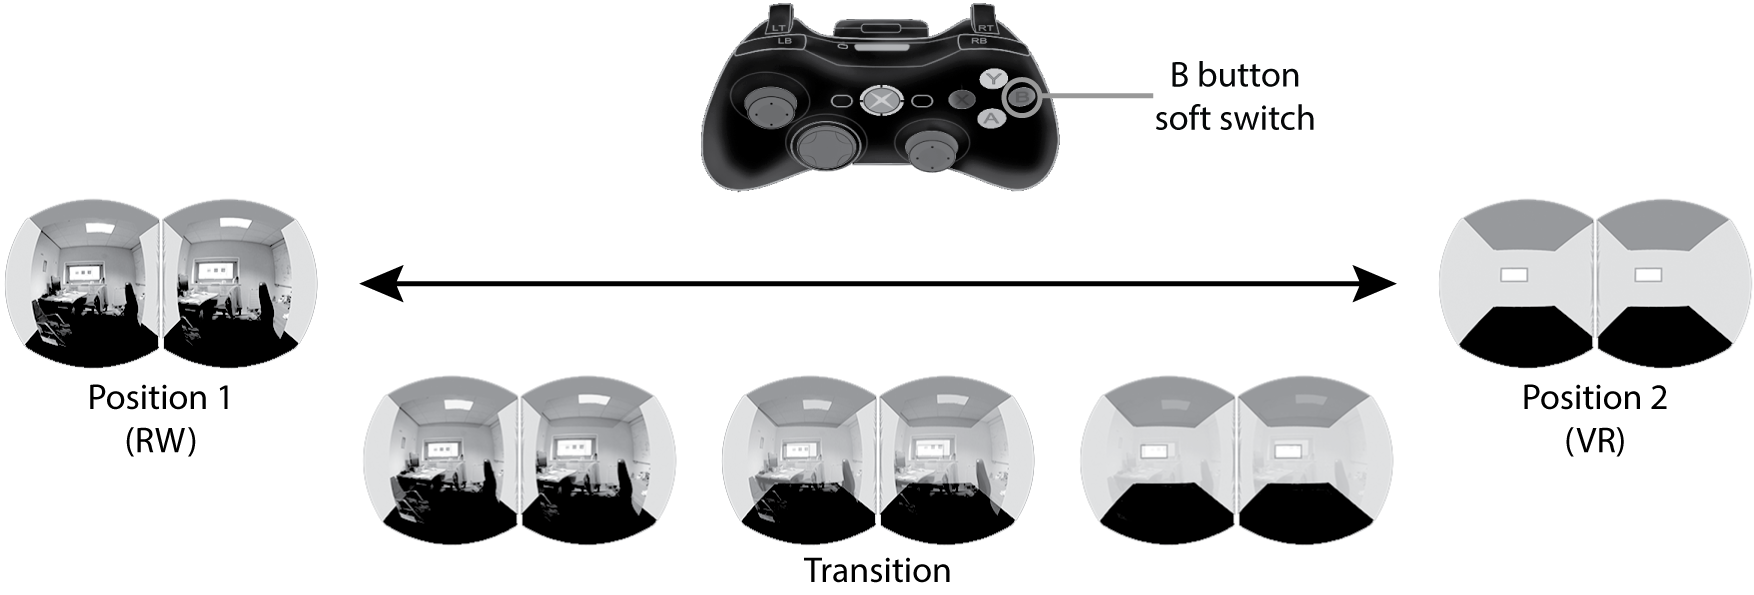
\includegraphics[width=\textwidth]{switching-soft-with-controller.png}
		\caption{Switch with linear interpolation.}
		\label{scenario12}
	\end{center}
\end{figure}

%=========================================================================================================

\subsubsection{Analogue selectable opacity}
The user pulls the right analogue trigger (\texttt{[RT]}) on the controller, where the position of the trigger maps directly to the opacity of the game objects that the webcam feeds are rendered upon. The user can choose to stop at any intermediary position that suits their needs, keeping the level of opacity of the webcam feeds at that position, as well as controlling the rate at which the visual stimuli from the RW environment fade (by changing how quickly they change their depression of the trigger). Pulling the trigger all the way in displays only visual stimuli from the VR environment, while releasing it completely displays only visual stimuli from the RW environment. The number of intermediary positions is limited only by the resolution of the trigger \& the encoding of the value.

This method allows the user to superimpose VR visual stimuli upon RW visual stimuli. This is similar, but not identical, to AR, as instead of displaying a small number of virtual objects upon the user's view of their RW environment, a complete VR environment is superimposed upon the user's view of their RW environment. Figure \ref{scenario2} illustrates this scenario.

\begin{figure}[h]
	\begin{center}
		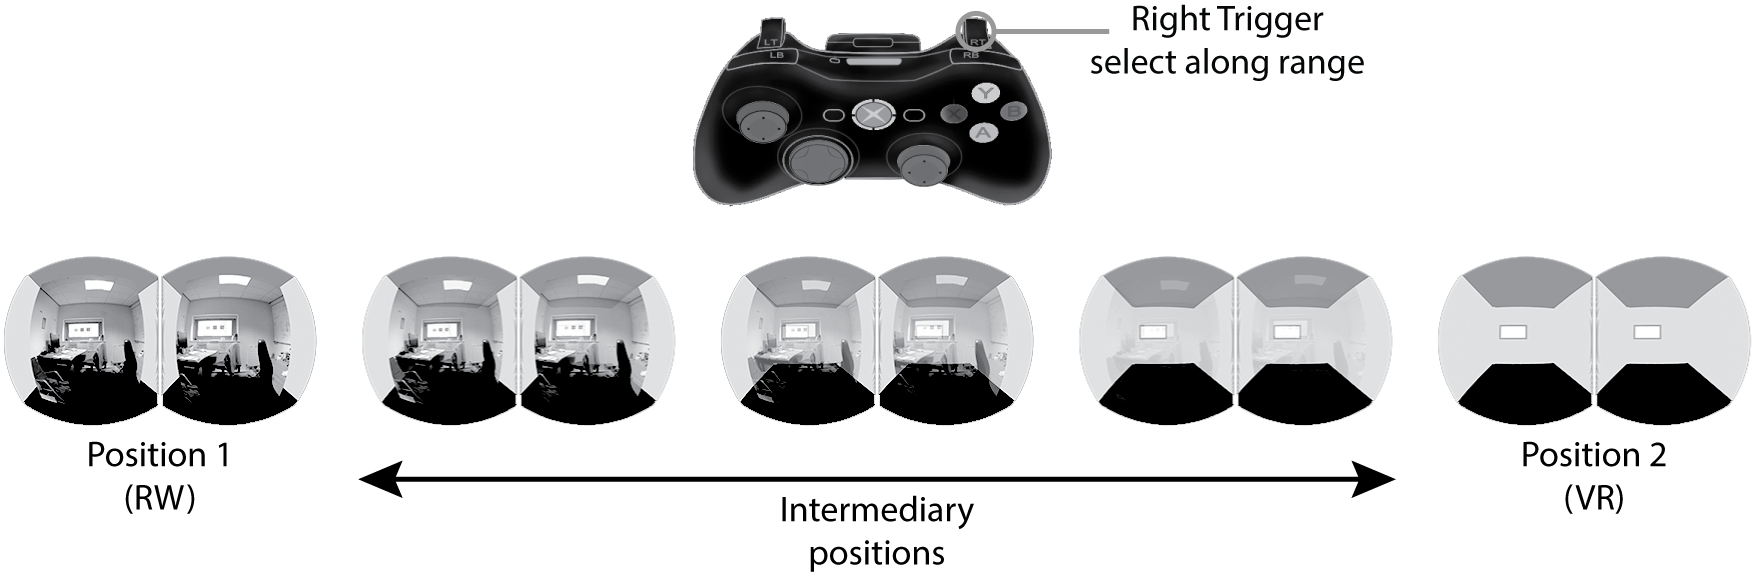
\includegraphics[width=.9\textwidth]{switching-analogue-with-controller.png}
		\caption{Analogue selectable opacity.}
		\label{scenario2}
	\end{center}
\end{figure}

%=========================================================================================================

\subsubsection{Periodic hard switches}
\label{subsub-periodic}
Independent or in addition to any of the previous scenarios, the visual stimuli displayed by the HMD switch from RW to VR at a set interval \& for a set amount of time. For example, every 3 seconds the stimuli switch from RW to VR for 0.2 of a second before switching back from VR to RW. Any user triggered transitions cause the interval timer to be reset, such that an `automated' switch will never occur after less time from a user triggered switch than the set interval. Automated transitions are disabled whilst \texttt{[RT]} is at all depressed. Figure \ref{scenariotimed} illustrates this scenario, where \texttt{i} represents the interval between switches \& \texttt{d} represents the duration of the switch from RW to VR.

\begin{figure}[h]
	\begin{center}
		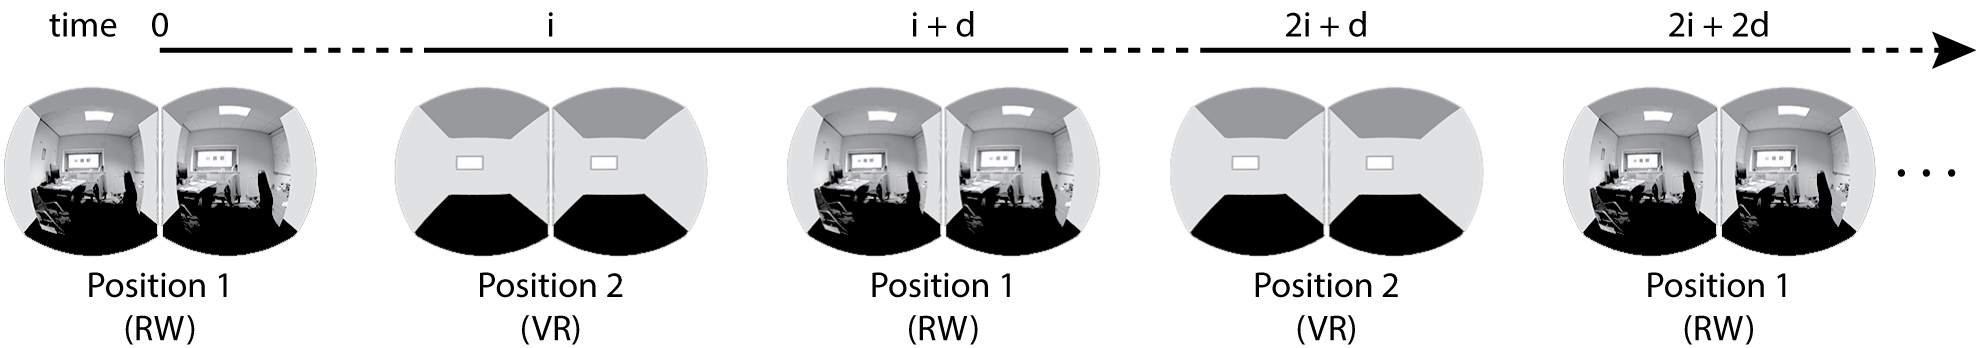
\includegraphics[width=\textwidth]{timed-switch.png}
		\caption{Periodic hard switches.}
		\label{scenariotimed}
	\end{center}
\end{figure}

%=========================================================================================================

\subsubsection{Reduced maximum opacity}
\label{subsub-baseopacity}
Independent or in addition to any of the previous scenarios, the maximum opacity of the game objects that the webcam feeds are rendered upon is reduced, such that the `default' position at which a transition has not been triggered (either by a button press, trigger movement or by a periodic switch) displays VR superimposed upon RW. Figure \ref{scenariobaseopacity} illustrates this scenario in combination with a hard switch (from section \ref{sub-hardswitch}) in which the user triggers hard switches between the default position of a superimposition of VR upon RW \& a position where only VR stimuli are present.

\begin{figure}[h]
	\begin{center}
		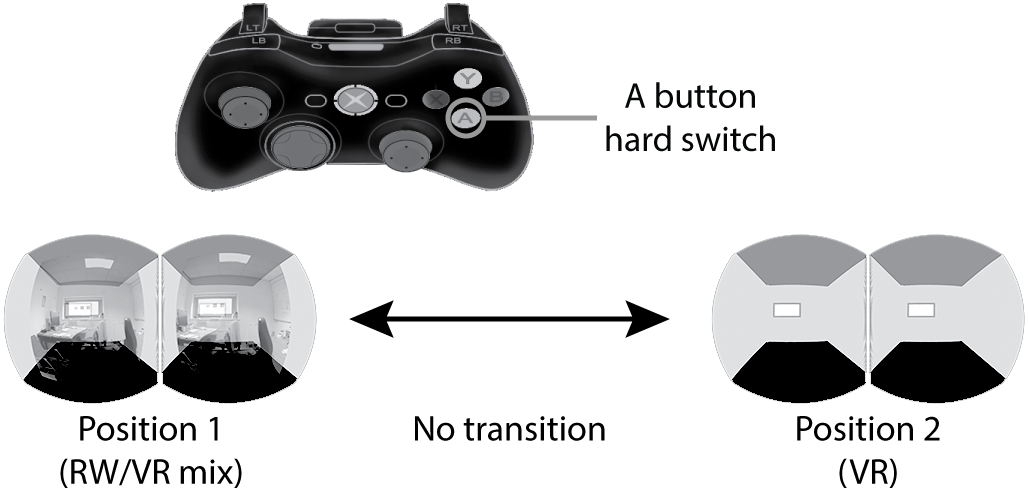
\includegraphics[width=0.7\textwidth]{base-opacity-hard-switch.png}
		\caption{Hard switch from reduced maximum opacity.}
		\label{scenariobaseopacity}
	\end{center}
\end{figure}

%=========================================================================================================





















%=========================================================================================================

%\textit{Two different buildings have been prepared for use with the Mirrorshades platform, with VR environments constructed \& the IndoorAtlas IPS deployed. The first is a modern building accompanied by a VR environment that closely depicts it in the present day. The second is a historic building accompanied by a VR environment that differs markedly from the present day, by depicting its state a point hundreds of years in the past.}

%\textit{In the first, participants will be given a simple task to complete which will encourage them to engage with the VR environment even though it presents a similar view to their RW environment. In the second scenario, participants will be prompted to engage in more free form exploration of their environments, comparing \& contrasting the markedly different VR environment with what they see around them in their RW environment.}

%\subsection{Jack Cole Building}
%The School of Computer Science Jack Cole building at St Andrews is a modern building, built in 2004. The VR environment accompanying the building is a fairly close representation of the building as it stands today. Figure \ref{jc_layout} shows the layout of the building \& the path that IndoorAtlas has been prepared for.

%There are four coloured panels (red, green, blue \& yellow) situated within the VR building upon walls, floor \& ceiling. Participants will be asked to remember in what order these panels are seen as they walk a lap of the building. This task is designed to encourage participants to switch between RW \& VR visual stimuli, even though the VR visual stimuli are very similar to those of the RW environment. This scenario is also intended to encourage participants to keep moving, rather than stopping at \& starting.

%\begin{figure}[h]
%	\begin{center}
%		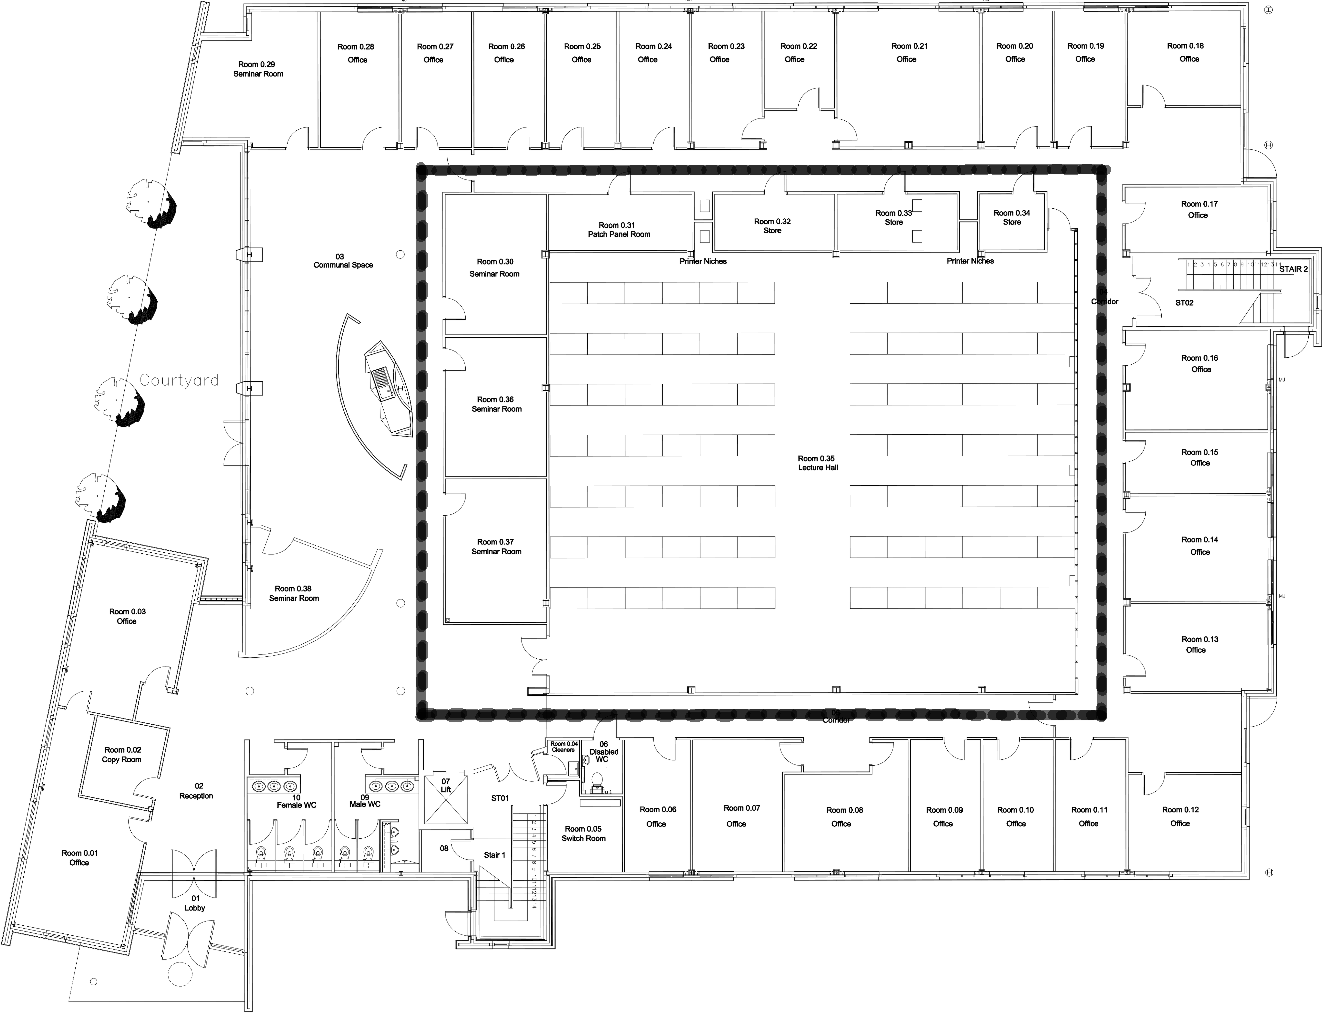
\includegraphics[width=0.7\textwidth]{JC_layout.png}
%		\caption{Floor plan of Jack Cole building, with IPS route.}
%		\label{jc_layout}
%	\end{center}
%\end{figure}

%=========================================================================================================